
\documentclass[reqno,11pt]{amsart}

%\usepackage{color,graphicx}
%\usepackage{mathrsfs,amsbsy}
\usepackage{amssymb}
\usepackage{amsmath}
\usepackage{amsfonts}
\usepackage{bm}
\usepackage{graphicx}
\usepackage{amsthm}
\usepackage{enumerate}
\usepackage[mathscr]{eucal}
\usepackage{float}
\usepackage{mathrsfs}
\usepackage{multicol}
\usepackage{multirow}
\usepackage[all,pdf]{xy}
\usepackage[a4paper,left=3cm,right=3cm]{geometry}
\usepackage[table,xcdraw]{xcolor} % before tikz-cd
\usepackage{tikz-cd}
\usepackage{hyperref}
\usepackage{quiver} 
\usepackage{changepage}
\usepackage{extpfeil} %for longer arrows
%\usepackage[notcite,notref]{showkeys}

% showkeys  make label explicit on the paper

\makeatletter
\@namedef{subjclassname@2010}{%
  \textup{2010} Mathematics Subject Classification}
\makeatother

\numberwithin{equation}{section}

\theoremstyle{plain}
\newtheorem{theorem}{Theorem}[section]
\newtheorem{lemma}[theorem]{Lemma}
\newtheorem{proposition}[theorem]{Proposition}
\newtheorem{corollary}[theorem]{Corollary}
\newtheorem{claim}[theorem]{Claim}
\newtheorem{defn}[theorem]{Definition}
\newtheorem{ques}[theorem]{Question}
\newtheorem*{fact}{Facts}
\newtheorem{eg}[theorem]{Example}

\theoremstyle{plain}
\newtheorem{thmsub}{Theorem}[subsection]
\newtheorem{lemmasub}[thmsub]{Lemma}
\newtheorem{corollarysub}[thmsub]{Corollary}
\newtheorem{propositionsub}[thmsub]{Proposition}
\newtheorem{defnsub}[thmsub]{Definition}

\numberwithin{equation}{section}


\theoremstyle{remark}

\newtheorem{remark}[theorem]{Remark}
\newtheorem{remarks}{Remarks}
\newtheorem*{remarkstar}{Remark}
\newtheorem*{problem}{Question}
\newtheorem*{answer}{Answer}
\newtheorem*{easyex}{Easy exercise}
%\renewcommand\thefootnote{\fnsymbol{footnote}}
%dont use number as footnote symbol, use this command to change

\DeclareMathOperator{\supp}{supp}
\DeclareMathOperator{\dist}{dist}
\DeclareMathOperator{\vol}{vol}
\DeclareMathOperator{\diag}{diag}
\DeclareMathOperator{\tr}{tr}
\DeclareMathOperator{\Img}{\operatorname{Im}}
\DeclareMathOperator{\Id}{\operatorname{Id}}
\DeclareMathOperator{\Rep}{\operatorname{Rep}}
\DeclareMathOperator{\Mod}{\operatorname{Mod}}
\DeclareMathOperator{\Hom}{\operatorname{Hom}}
\DeclareMathOperator{\Ext}{\operatorname{Ext}}
\DeclareMathOperator{\gldim}{\operatorname{gl.dim}}
\DeclareMathOperator{\projdim}{\operatorname{proj.dim}}
\DeclareMathOperator{\injdim}{\operatorname{inj.dim}}
\DeclareMathOperator{\dimv}{\operatorname{\underline{\mathbf{dim}}}}
\DeclareMathOperator{\SL}{\operatorname{SL}}
\DeclareMathOperator{\PGL}{\operatorname{PGL}}
\DeclareMathOperator{\Flagd}{\operatorname{Flag}_{d}}
\DeclareMathOperator{\Flagdstr}{\operatorname{Flag}_{d,str}}
\newcommand{\Gr}{\operatorname{Gr}}
\newcommand{\Grr}{\operatorname{Gr}}
\newcommand{\Grq}{\operatorname{Gr}^{KQ}}
\newcommand{\Flag}[1]{\operatorname{Flag}_{#1}}
\newcommand{\Flagstr}[1]{\operatorname{Flag}_{#1,str}}
\newcommand{\dimvec}[1]{#1}
\newcommand{\ord}{\operatorname{ord}}
\newcommand{\orde}{\operatorname{ord}_e }
\newcommand{\representation}[2]{\genfrac{}{}{0pt}{3}{\phantom{000}#2\phantom{00}}{#1}}
\newcommand{\Spec}{\operatorname{Spec}}
\newcommand{\Proj}{\operatorname{Proj}}
\newcommand{\Pic}{\operatorname{Pic}}
\newcommand{\Coh}{\operatorname{Coh}}
\newcommand{\Psh}{\operatorname{Psh}}
\newcommand{\Schk}{\operatorname{Sch}_{k}}
\newcommand{\SchX}{\operatorname{Sch}_{X}}
\newcommand{\Set}{\operatorname{Set}}
\newcommand{\Ob}{\operatorname{Ob}}
\newcommand{\Mor}{\operatorname{Mor}}
\newcommand{\Hilb}{\operatorname{Hilb}}
\newcommand{\Quot}{\operatorname{Quot}}
\newcommand{\Sym}{\operatorname{Sym}}
\setlength\intextsep{0cm}
\setlength\textfloatsep{0cm}
\begin{document}
\date{}

\title
{Moduli in Algebraic Geometry}


\author{Xiaoxiang Zhou}
\address{School of Mathematical Sciences\\
University of Bonn\\
Bonn, 53115\\ Germany\\} 
\email{email:xx352229@mail.ustc.edu.cn}





\begin{abstract}
In this personal survey, we conclude the definitions of moduli functors in the algebraic geometry. Most of the results are in the black box, so it's very possible that they're wrong. And also I'm not responsible for the completeness of the whole theory. However, I'm still happy to improve this document, and make it better over time.
\end{abstract}

\setcounter{tocdepth}{1}
\maketitle
\tableofcontents
%%%%%%%%%%%%%%%%%%%%%%%%%%%%%%%%%%%%%%%%%%%%%%%%%%%%%%%%%%%%%%%%%%%%%%%%%%%%%%%%%%%%%%%%%%%%%
\section{Goal and related concepts}
The personal survey is motivated by the three courses in Bonn: \href{https://johannesschmitt.gitlab.io/moduli_of_curves}{``the moduli space of curves"}, \href{https://www.math.uni-bonn.de/people/mihatsch/21u22\%20WS/moduli/}{``moduli of elliptic curves"} and \href{https://www.math.uni-bonn.de/people/ydutta/v5a4}{``moduli of vector bundles"}. I would also highly recommend the course \href{https://userpage.fu-berlin.de/hoskins/moduli_and_GIT.html}{``Moduli and GIT"} in Freie Universität Berlin. I want to construct my personal understanding on the moduli, and find out the details I missed in the courses. 

``Some mathematicians are birds, others
are frogs." This document is devoted to those ``birds" from a ``frog" who gets stuck in the mud.
\subsection{Conventions and Notations}
In this survey,  $\Schk$ is denoted as the category of \textbf{locally Noetherian} schemes over $k$.
\subsection{Representable functor}
In this subsection we would follow on \cite[Definition 2.2.1]{huybrechts2010geometry} in full generality, but you can always think 
$$\mathcal{C}=\Schk \qquad \mathcal{C}'=\operatorname{Functor} (\Schk^{op},\Set)$$
to visualize the statement, and you can refer to \cite[6.6.2]{FOAG} to see basic examples.
\begin{defn}[Functor category]
Fix a category $\mathcal{C}$, we define the corresponding functor category $\mathcal{C}'$ as follows:
% https://q.uiver.app/?q=WzAsMixbMCwwLCJcXG1hdGhjYWx7Q31ee29wfSJdLFsxLDAsIlxcU2V0Il0sWzAsMSwiIiwwLHsiY3VydmUiOjF9XSxbMCwxLCIiLDIseyJjdXJ2ZSI6LTF9XSxbMywyLCIiLDIseyJzaG9ydGVuIjp7InNvdXJjZSI6MjAsInRhcmdldCI6MjB9fV1d
$$\Ob(\mathcal{C}'):=\left\{  \text{functors }\mathcal{C}^{op}\longrightarrow \Set \right\} \qquad \Mor(\mathcal{C}'):=\left\{ \text{natural trans }
\begin{tikzcd}
	{\mathcal{C}^{op}} & \Set
	\arrow[""{name=0, anchor=center, inner sep=0}, curve={height=9pt}, from=1-1, to=1-2]
	\arrow[""{name=1, anchor=center, inner sep=0}, curve={height=-9pt}, from=1-1, to=1-2]
	\arrow[shorten <=2pt, shorten >=2pt, Rightarrow, from=1, to=0]
\end{tikzcd}
\right\}$$
In brief, $\mathcal{C}'=\operatorname{Functor} (\mathcal{C}^{op},\Set)$.\footnote{From  \href{https://userpage.fu-berlin.de/hoskins/moduli_and_GIT.html}{here} we can also write $\mathcal{C}'=\Psh(C)$, notice that here it is the presheaf on \textbf{category}, not on a specific scheme $X/k$.}
\end{defn}
\begin{proposition}
We have a canonical functor 
$$\iota: \mathcal{C} \longrightarrow \mathcal{C}' \qquad X \longmapsto h_X:=\Mor_{\mathcal{C}}(-,X)$$ which embeds $\mathcal{C}$ as a full subcategory of $\mathcal{C}'$.\footnote{$h_X$ is called the functor of points of a scheme $X$ from  \href{https://userpage.fu-berlin.de/hoskins/moduli_and_GIT.html}{here}. For example, $h_X(\Spec \mathbb{Q})=X(\mathbb{Q})$ gives us the set of rational points in $X$(under certain conditions). Notice that $h_{-}(-)$ is a bifunctor.}
\end{proposition}
\begin{proof}
Recall that the Yoneda's lemma gives us the isomorphism
$$\Mor_{\mathcal{C}'}(h_X,F)\cong F(X).$$
\end{proof}
\begin{defn}[Representable functor]\label{def:repfctor}
The functor $F\in \Ob(\mathcal{C}')$ is called represented by $X$ if $F\cong h_X$.
\end{defn}
From this proposition, we can always view the object as some functor satisfying some properties. we get three advantages from this point of view:
\begin{itemize}
\item It's easy to see rational points and complex points;
\item We can define scheme canonically, without explicit constructions;
\item We can enlarge our area of research, and think them as the defective schemes. We will see some reasonable functors which is represented not by schemes, but by stacks.
\end{itemize}
\subsection{Corepresentable functor}
This is the concept "dual to" the representable functor. To motivate, we begin with the equivalent definition of representable functor:
\begin{defn}[Representatable functor, equivalent definition]
A functor $F\in \Ob(\mathcal{C}')$ is represented by $X \in \Ob(C)$ if $F$ satisfies the following universal properties:
\begin{itemize}
\item There exists a morphism $\eta^{-1}:h_X \longrightarrow F$ in $\Mor_{\mathcal{C}'}(h_X,F)$;
\item For any object $X' \in \Ob(\mathcal{C})$ and morphism $\alpha':h_{X'}\longrightarrow F$ in $\Mor_{\mathcal{C}'}(h_{X'},F)$, there exists an unique morphism $\beta \in \Mor_{\mathcal{C}}(X',X)$ such that $\alpha'=\eta^{-1} \circ h_{\beta}$.
% https://q.uiver.app/?q=WzAsNSxbMCwwXSxbMSwwLCJoX3tYJ30iXSxbMSwxLCJoX3tYfSJdLFsyLDBdLFsyLDEsIkYiXSxbMSwyLCJcXGV4aXN0IFxcLCEgXFwsaF97XFxiZXRhfSIsMix7ImNvbG91ciI6WzM1OCwxMDAsNTBdLCJzdHlsZSI6eyJib2R5Ijp7Im5hbWUiOiJkYXNoZWQifX19LFszNTgsMTAwLDUwLDFdXSxbMiw0LCJcXGFscGhhIiwyXSxbMSw0LCJcXGFscGhhJyJdXQ==
$$\begin{tikzcd}
	{} & {h_{X'}} & {} \\
	& {h_{X}} & F
	\arrow["{\exists \,! \,h_{\beta}}"', color={rgb,255:red,255;green,0;blue,8}, dashed, from=1-2, to=2-2]
	\arrow["\eta^{-1}"', from=2-2, to=2-3]
	\arrow["{\alpha'}", from=1-2, to=2-3]
\end{tikzcd}$$
\end{itemize}
\end{defn}
This definition is equivalent to the Definition \ref{def:repfctor} since \footnote{The middle isomorphism comes from the universal property, while the two equalities come from the Yoneda's lemma.}
$$h_X(X')=\Mor_{\mathcal{C}}(X',X) \cong \Mor_{\mathcal{C}'}(h_{X'},F) =F(X') \text{ for any } X'\in \Ob(\mathcal{C})$$
thus the functor $\eta^{-1}: h_X \longrightarrow F$ is an isomorphism.
\begin{defn}[Corepresentable functor]
A functor $F\in \Ob(\mathcal{C}')$ is corepresented by $X \in \Ob(C)$ if $F$ satisfies the following universal properties:
\begin{itemize}
\item There exists a morphism $\eta:F \longrightarrow h_X$ in $\Mor_{\mathcal{C}'}(F,h_X)$;
\item For any object $X' \in \Ob(\mathcal{C})$ and morphism $\alpha':F\longrightarrow h_{X'}$ in $\Mor_{\mathcal{C}'}(F,h_{X'})$, there exists an unique morphism $\beta \in \Mor_{\mathcal{C}}(X,X')$ such that $\alpha'=h_{\beta} \circ \eta$.
% https://q.uiver.app/?q=WzAsMyxbMCwwLCJGIl0sWzEsMCwiaF9YIl0sWzEsMSwiaF97WCd9Il0sWzAsMSwiXFxhbHBoYSJdLFsxLDIsIlxcZXhpc3QgXFwsISBcXCxoX3tcXGJldGF9IiwwLHsiY29sb3VyIjpbMzU4LDEwMCw1MF0sInN0eWxlIjp7ImJvZHkiOnsibmFtZSI6ImRhc2hlZCJ9fX0sWzM1OCwxMDAsNTAsMV1dLFswLDIsIlxcYWxwaGEnIiwyXV0=
$$\begin{tikzcd}
	F & {h_X} \\
	& {h_{X'}}
	\arrow["\eta", from=1-1, to=1-2]
	\arrow["{\exists \,! \,h_{\beta}}", color={rgb,255:red,255;green,0;blue,8}, dashed, from=1-2, to=2-2]
	\arrow["{\alpha'}"', from=1-1, to=2-2]
\end{tikzcd}$$
\end{itemize}
\end{defn}
\begin{defn}[Universal corepresentable functor]

\end{defn}
\begin{proposition}
Suppose a functor $F\in \Ob(\mathcal{C}')$ is corepresented by $X \in \Ob(C)$, then it is represented by $X$ if and only if $\eta:F \longrightarrow h_X$ is a $\mathcal{C}'$-isomorphism.
\end{proposition}
\subsection{Coarse moduli space}
You need to see the definition of the naive moduli problem, extended moduli problem, moduli functor, fine moduli space and corresponding universal family from  \href{https://userpage.fu-berlin.de/hoskins/moduli_and_GIT.html}{here}. I don't want to copy, and it's well-written.

The following example will check if you really understand these concepts.
\begin{eg}[$\mathcal{M}_{0,3}$ is represented by one point $\Spec k$]\label{eg:M03}\

\textbf{Naive moduli problem} $(\mathcal{A},\sim)$:
$$\mathcal{A}:=\left\{(p_1,p_2,p_3)  \;\middle|\; p_i \in \mathbb{P}_k^1(k) \text{ are distinct } \right\}$$
$$(p_1,p_2,p_3) \sim (q_1,q_2,q_3) \Longleftrightarrow \exists \, \gamma \in \PGL_2(k) \text{ s.t. } q_i=\gamma(p_i)$$

\textbf{Extended moduli problem} $(\mathcal{A}_S,\sim_S)$ + pullback: \textcolor{gray}{$(S \in \Ob(\Schk))$}
$$\mathcal{A}_S:=\left\{(X,\pi,\sigma_1,\sigma_2,\sigma_3)  \;\middle|\; \begin{aligned}
&\\[-5mm]
&X \in \Ob(\Schk)\\[-1mm]
&\pi:X \longrightarrow S \text{ proper flat and }\pi^{-1}(p)\cong\mathbb{P}_{\kappa(p)}^1 \\[-1mm]
&\sigma_i:S \longrightarrow X \text{ pairwise disjoint sections of }\pi
\end{aligned}
 \right\}$$
 
 $(X,\pi,\sigma_1,\sigma_2,\sigma_3) \sim_S (X',\pi',\sigma_1',\sigma_2',\sigma_3')$ if there exists an isomorphism $f:X \longrightarrow X'$ such that the following diagrams commute:
   % https://q.uiver.app/?q=WzAsNixbMCwwLCJYIl0sWzIsMCwiWCciXSxbMSwxLCJTIl0sWzMsMCwiWCJdLFs0LDEsIlMiXSxbNSwwLCJYJyJdLFszLDUsImYiXSxbNCw1LCJcXHNpZ21hX2knIiwyXSxbNCwzLCJcXHNpZ21hX2kiXSxbMCwyLCJcXHBpIiwyXSxbMSwyLCJcXHBpJyJdLFswLDEsImYiXV0=
   \[\begin{tikzcd}[column sep=3mm]
   	X && {X'} &[20mm] X && {X'} \\
   	& S &&& S
   	\arrow["f", from=1-4, to=1-6]
   	\arrow["{\sigma_i'}"', from=2-5, to=1-6]
   	\arrow["{\sigma_i}", from=2-5, to=1-4]
   	\arrow["\pi"', from=1-1, to=2-2]
   	\arrow["{\pi'}", from=1-3, to=2-2]
   	\arrow["f", from=1-1, to=1-3]
   \end{tikzcd}\]
   
   For a map $f:T \longrightarrow S$, the pullback $f^*$ is defined by
   $$f^*:\mathcal{A}_S \longrightarrow \mathcal{A}_T \qquad (X,\pi,\sigma_1,\sigma_2,\sigma_3) \longmapsto (X_T,\pi_T,\sigma_{1,T},\sigma_{2,T},\sigma_{3,T})$$
   where $X_T$, $\pi_T$ are defined as fiber product, and $\sigma_{i,T}$ are defined by the universal property of fiber product, as follows:
   % https://q.uiver.app/?q=WzAsOSxbMCwxLCJYX1QiXSxbMSwxLCJYIl0sWzAsMiwiVCJdLFsxLDIsIlMiXSxbMywxLCJYX1QiXSxbMywyLCJUIl0sWzQsMiwiUyJdLFs0LDEsIlgiXSxbMiwwLCJUIl0sWzAsMiwiXFxwaV9UIiwyXSxbMiwzLCJmIl0sWzEsMywiXFxwaSJdLFs0LDUsIlxccGlfVCIsMl0sWzUsNiwiZiJdLFs3LDYsIlxccGkiLDJdLFs0LDddLFs4LDcsIlxcc2lnbWFfaSBcXGNpcmMgZiIsMCx7ImN1cnZlIjotMn1dLFs4LDQsIlxcZXhpc3RzIFxcLCFcXCwgXFxzaWdtYV97aSxUfSAiLDAseyJsYWJlbF9wb3NpdGlvbiI6OTAsImNvbG91ciI6WzAsMTAwLDUwXSwic3R5bGUiOnsiYm9keSI6eyJuYW1lIjoiZGFzaGVkIn19fSxbMCwxMDAsNTAsMV1dLFs4LDUsIlxcSWRfVCIsMix7ImN1cnZlIjoyfV0sWzYsNywiXFxzaWdtYV97aX0iLDIseyJjdXJ2ZSI6MSwic3R5bGUiOnsiYm9keSI6eyJuYW1lIjoiZGFzaGVkIn19fV0sWzAsMV0sWzAsMywiIiwxLHsic3R5bGUiOnsibmFtZSI6ImNvcm5lciJ9fV0sWzQsNiwiIiwxLHsic3R5bGUiOnsibmFtZSI6ImNvcm5lciJ9fV1d
   \[\begin{tikzcd}
   	&&[15mm] T&[-6mm] \\[-6mm]
   	{X_T} & X && {X_T} & X \\
   	T & S && T & S
   	\arrow["{\pi_T}"', from=2-1, to=3-1]
   	\arrow["f", from=3-1, to=3-2]
   	\arrow["\pi", from=2-2, to=3-2]
   	\arrow["{\pi_T}"', from=2-4, to=3-4]
   	\arrow["f", from=3-4, to=3-5]
   	\arrow["\pi"', from=2-5, to=3-5]
   	\arrow[from=2-4, to=2-5]
   	\arrow["{\sigma_i \circ f}", curve={height=-12pt}, from=1-3, to=2-5]
   	\arrow["{\exists \,!\, \sigma_{i,T} }"{pos=1.12}, color=red, dashed, from=1-3, to=2-4]
   	\arrow["{\Id_T}"', curve={height=12pt}, from=1-3, to=3-4]
   	\arrow["{\sigma_{i}}"', curve={height=6pt}, dashed, from=3-5, to=2-5]
   	\arrow[from=2-1, to=2-2]
   	\arrow["\ulcorner"{anchor=center, pos=0.125}, draw=none, from=2-1, to=3-2]
   	\arrow["\ulcorner"{anchor=center, pos=0.125}, draw=none, from=2-4, to=3-5]
   \end{tikzcd}\]
 \begin{adjustwidth}{10mm}{0em}
 \begin{remarkstar}
 We can always view the point $p \in S$ as an affine scheme of its residue field. So the two conditions below are equivalent:
 \begin{equation*}
 \begin{aligned}
  &\pi^{-1}(p)\cong\mathbb{P}_{\kappa(p)}^1& & \text{ for any } p \in S  \\ 
  &\pi^{-1}(\Spec L)\cong \mathbb{P}_{L}^1& & \text{ for any } \Spec L \hookrightarrow S  \\ 
 \end{aligned}
 \end{equation*}
 \end{remarkstar}
 \begin{remarkstar}
 In some textbooks, they require $\pi:X \longrightarrow S$ to be a smooth, proper, surjective, locally finitely presented (l.f.p.)
 morphism of relative dimension $\leqslant 1$ with geometric fibres isomorphic to $\mathbb{P}^1$. These extra conditions are automatically satisfied, since
 % https://q.uiver.app/?q=WzAsNixbMCwwLCJcXGJ1bGxldCJdLFsxLDAsIlxcdGV4dHtzdXJqZWN0aXZlfSJdLFsxLDEsIlxcYnVsbGV0Il0sWzAsMSwiXFxidWxsZXQiXSxbMSwyLCJcXGJ1bGxldCJdLFswLDIsIlxcYnVsbGV0Il0sWzAsMV0sWzAsMl0sWzMsMl0sWzMsNF0sWzUsNF1d
 \[\begin{tikzcd}[/tikz/column 1/.append style={anchor=base east},/tikz/column 2/.append style={anchor=base west}, column sep=3cm, row sep=-2mm,start anchor=east,end anchor=west]
 	\pi^{-1}(p)\cong\mathbb{P}_{\kappa(p)}^1 & {\text{surjective}} \\
 	{\text{proper}} & {\text{relative dimension $\leqslant 1$}} \\
 	{\text{locally Noetherian}} & {\text{locally finitely presented}}
 	\arrow[from=1-1, to=1-2]
 	\arrow[from=1-1, to=2-2]
 	\arrow[from=2-1, to=2-2]
 	\arrow[from=2-1, to=3-2]
 	\arrow[from=3-1, to=3-2]
 \end{tikzcd}\]
 and by \cite[25.2.2]{FOAG}, flat + fiberwise $\mathbb{P}^1$ + l.f.p. $\Rightarrow$ smooth. 
 
 \end{remarkstar}
\begin{problem}\hspace{1cm}

Can we find $(X,\pi,\sigma_1,\sigma_2,\sigma_3)$ satisfying all conditions in $\mathcal{A}_S$ except $\pi$ is seperated? 

Can we find $(X,\pi,\sigma_1,\sigma_2,\sigma_3)$ satisfying all conditions in $\mathcal{A}_S$ except $\pi$ is flat?
\end{problem}
\begin{easyex}\hspace{1cm}

Verify that $(\mathcal{A}_S,\sim_S)$ and pullback satisfy (i)-(iv) in \cite[Definition 2.10]{moduliGIT}.
\end{easyex}



 \end{adjustwidth}



\textbf{Moduli functor} $\mathcal{M}_{0,3}$:
The moduli functor $\mathcal{M}_{0,3}: \Schk^{op}\longrightarrow \Set$ is defined as
$$\mathcal{M}_{0,3}(S)=\mathcal{A}_S/\sim_S \qquad \mathcal{M}_{0,3}(f:T\longrightarrow S)=f^*: \mathcal{A}_S/\sim_S \longrightarrow \mathcal{A}_T/\sim_T.$$
\vspace{-1.1cm}
\begin{adjustwidth}{10mm}{0em}

\begin{problem}\hspace{1cm}

Why is the moduli functor $\mathcal{M}_{0,3}$ represented by $\Spec k$?
\end{problem}
\begin{answer}\hspace{1cm}

Yes, but it's pretty hard to prove it. The proof of \cite[Proposition 4.1]{modulicurve} uses \cite[Proposition 4.2]{modulicurve} whose proof is quite technical.

Actually we construct the natural functor $\eta^{-1}:h_{\Spec k} \longrightarrow \mathcal{M}_{0,3}$ by
$$\eta^{-1}_S:h_{\Spec k}(S) \longrightarrow \mathcal{M}_{0,3}(S) \qquad [S \rightarrow \Spec k] \longmapsto (\mathbb{P}_S^1=\mathbb{P}_k^1 \times_k S, pr_1,0,1,\infty)$$
and then verify that $\eta^{-1}_S$ is an isomorphism.
\end{answer}
\end{adjustwidth}
\textbf{Universal family}:
By \cite[Definition 2.16]{moduliGIT}, the universal family is $(\mathbb{P}_k^1, \pi,0,1,\infty)$.

\end{eg}

coarse moduli space and some related concepts. 
\subsection{Stack}
We need to define stack, algebraic stack, Deligne-Munford stack and some related concepts.
\subsection{Goal}
???

We will frequently use the quotient. Here is the list of quotients we've already seen:
\begin{itemize}
\item (We could begin at topology:quotient by a subset) linear space-> Abelian category,group,ring(Notice that for this item, we don't take quotient by a group, so sometimes it looks easier)
\item topology(This gives us an categorical quotient!)
\item manifold
\item scheme(Categorical quotient; GIT quotient)
\end{itemize}
%%%%%%%%%%%%%%%%%%%%%%%%%%%%%%%%%%%%%%%%%%%%%%%%%%%%%%%%%%%%%%%%%%%%%%%%%%%%%%%%%%%%%%%%%%%%%
\section{Basic object}
In this section, we present some algebraic geometric objects which can be viewed as moduli.

Here is a picture showing the relationships of these objects:
% https://tikzcd.yichuanshen.de/#N4Igdg9gJgpgziAXAbVABwnAlgFyxMJZABgBpiBdUkANwEMAbAVxiRAB12BbOnACwBGA4AAUAvgDUQY0uky58hFGQCMVWoxZtOPfkNFidvPgGNGwAGJjpskBmx4CRFaTXV6zVog7sA4gCcACn9SCQBKGzkHRWdSACZ1Dy1vTgBFJggcSLt5RyUSeMTNLx8ACSwGAWz7BScUOML3Yu12CwY6AHMoQPDpdRgoDvgiUAAzfwguJDIQHAgkFRkxianEGbmkOKWQccnN6g3EAGZt3dWXWfnj05WkABYDq5PbM-3LpABWMQoxIA
\[\begin{tikzcd}[row sep={12mm,between origins}, column sep={15mm,between origins}]
\mathbb{P}V \arrow[d] \arrow[rd] &                                 &           \\
\mathbb{P}\mathcal{F} \arrow[rd] & {\Gr(r,V)} \arrow[d] \arrow[rd] &           \\
\Hilb \arrow[r]                  & \Quot                           & \Flagd(V)
\end{tikzcd}\]
\subsection{Projective space}
We begin with a basic extended moduli problem, and then gradually make some variations.
\begin{eg}[Moduli of line bundle with base-point-free sections is represented by $\mathbb{P}_k^n$]
Fix $n \geqslant 0$, we define a moduli problem:
$$\mathcal{A}_S:=\left\{(\mathcal{L},s_0,\ldots,s_n)  \;\middle|\; \begin{aligned}
&\\[-5mm]
&\mathcal{L} \in \Pic(S)\\[-1mm]
& s_i \in \Gamma(S,\mathcal{L}) \text{ with no common zero }
\end{aligned}
 \right\}$$
 
  $(\mathcal{L},s_0,\ldots,s_n) \sim_S (\mathcal{L}',s_0',\ldots,s_n')$ if there exists an isomorphism of line bundles $\phi:\mathcal{L} \longrightarrow \mathcal{L}'$ such that $\phi(S):\Gamma(S,\mathcal{L}) \longrightarrow \Gamma(S,\mathcal{L}')$ sends $s_i$ to $s_i'$.
  
  For a map $f:T \longrightarrow S$, the pullback $f^*$ is defined by
     $$f^*:\mathcal{A}_S \longrightarrow \mathcal{A}_T \qquad (\mathcal{L},s_0,\ldots,s_n) \longmapsto (f^*\mathcal{L},f^*s_0,\ldots,f^*s_n)$$
     
By \cite[15.3.F, 16.4.1]{FOAG}, the moduli functor defined by this extended moduli problem is represented by $\mathbb{P}_k^n$.
\end{eg}
We also have the coordinate-free version.
\begin{eg}[{Coordinate-free projective space $\mathbb{P}V^{\vee}=\Proj(\Sym^{\bullet} V)$, see \cite[4.5.12]{FOAG}}]
Fix a $k$-vector spcace $V$ of finite dimension. We define a moduli problem:
$$\mathcal{A}_S:=\left\{(\mathcal{L},\lambda)  \;\middle|\; \begin{aligned}
&\\[-5mm]
&\mathcal{L} \in \Pic(S)\\[-1mm]
& \lambda:V \longrightarrow \Gamma(S,\mathcal{L}) \text{ is base-point-free }
\end{aligned}
 \right\}$$
 
   $(\mathcal{L},\lambda) \sim_S (\mathcal{L}',\lambda')$ if there exists an isomorphism of line bundles $\phi:\mathcal{L} \longrightarrow \mathcal{L}'$ such that $\lambda'=\phi(S) \circ \lambda$.
   
   For a map $f:T \longrightarrow S$, the pullback $f^*$ is defined by
      $$f^*:\mathcal{A}_S \longrightarrow \mathcal{A}_T \qquad (\mathcal{L},\lambda) \longmapsto \big(f^*\mathcal{L},f^*\circ \lambda:V \rightarrow \Gamma(T,f^*\mathcal{L})\big)$$
      
      By \cite[16.4.E]{FOAG}, the moduli functor defined by this extended moduli problem is represented by $\mathbb{P}V^{\vee}$.
\end{eg}
Now we generalize it to the projective bundle, for this we should fix a scheme $X \in \Ob(\Schk)$ and a locally free coherent sheaf $\mathcal{F} \in \Coh(X)$, and consider the moduli problem in the category $\SchX$ of locally Noetherian schemes over $X$, rather than $\Schk$.

\begin{eg}[{Projective bundle\footnote{There is an notational abuse in \cite{FOAG}. From my personal point of view, it's better to replace $\mathbb{P}\mathcal{F}$ with $\mathbb{P}\mathcal{F}^{\vee}$ or $\mathbb{P}V^{\vee}$ with $\mathbb{P}V$ to make symbols consistent. } $\mathbb{P}\mathcal{F}=\Proj(\Sym^{\bullet} \mathcal{F})$, see \cite[17.2.3]{FOAG}}]\hspace{1cm}

For $(S,\pi_S: S \longrightarrow X) \in \Ob(\SchX)$, we define a moduli problem:
$$\mathcal{A}_S:=\left\{(\mathcal{L},\lambda)  \;\middle|\; \begin{aligned}
&\\[-5mm]
&\mathcal{L} \in \Pic(S)\\[-1mm]
& \lambda:\pi_S^* \mathcal{F} \xtwoheadrightarrow{\hspace{2mm}}  \mathcal{L}
\end{aligned}
 \right\}$$
 
   $(\mathcal{L},\lambda) \sim_S (\mathcal{L}',\lambda')$ if there exists an isomorphism of line bundles $\phi:\mathcal{L} \longrightarrow \mathcal{L}'$ such that $\lambda'=\phi \circ \lambda$.
   
   For a map $f:T \longrightarrow S$, the pullback $f^*$ is defined by
      $$f^*:\mathcal{A}_S \longrightarrow \mathcal{A}_T \qquad (\mathcal{L},\lambda) \longmapsto \big(f^*\mathcal{L},f^* \lambda:\pi_T^*\mathcal{F} \twoheadrightarrow f^*\mathcal{L}\big)$$
      
      By \cite[Proposition 7.12]{hartshorne2013algebraic}, the moduli functor defined by this extended moduli problem is represented by $\mathbb{P}\mathcal{F}$.
\end{eg}

Finally, there is also "another" natural moduli problem of $\mathbb{P}_k^n$, see \cite[Example 2.4]{modulicurve}. For the convinience of comparison with Grassmannian, we exhibit it and make some small variations here.\footnote{The reason of the variation is already explained in \cite[16.7, page 442]{FOAG}.}

\begin{eg}[{Moduli of lines through the origin in $\mathbb{A}_k^{n+1}$ is represented by $\mathbb{P}_k^n$}]
For $n \geqslant 0$, we define a moduli problem:
$$\mathcal{A}_S:=\left\{(\mathcal{L},\pi)  \;\middle|\; \begin{aligned}
&\\[-5mm]
&\mathcal{L} \in \Pic(S)\\[-1mm]
& \pi:\mathcal{O}_S^{\oplus n+1} \xtwoheadrightarrow{\hspace{2mm}}  \mathcal{L}
\end{aligned}
 \right\}$$
 
   $(\mathcal{L},\pi) \sim_S (\mathcal{L}',\pi')$ if there exists an isomorphism of line bundles $\phi:\mathcal{L} \longrightarrow \mathcal{L}'$ such that $\pi'=\phi \circ \pi$.
   
   For a map $f:T \longrightarrow S$, the pullback $f^*$ is defined by
      $$f^*:\mathcal{A}_S \longrightarrow \mathcal{A}_T \qquad (\mathcal{L},\pi) \longmapsto \big(f^*\mathcal{L},f^* \pi:\mathcal{O}_T^{\oplus n+1} \twoheadrightarrow f^*\mathcal{L}\big)$$
      
      By \cite[Proposition 7.12]{hartshorne2013algebraic}, the moduli functor defined by this extended moduli problem is represented by $\mathbb{P}\mathcal{F}$.
\end{eg}
\subsection{Grassmannian}
It's well-written in \cite[16.7]{FOAG}. We just exhibit(copy) the moduli problem and make a short remark about the existence proof (prove the representability without explicite construction of the scheme)
\begin{eg}[{Grassmannian $\Gr(k,n)$}]
For $n \geqslant k \geqslant 0$, we define a moduli problem:
$$\mathcal{A}_S:=\left\{(\mathcal{F},\pi)  \;\middle|\; \begin{aligned}
&\\[-5mm]
&\mathcal{F} \in \Coh(S) \text{ locally free of rank $k$ }\\[-1mm]
& \pi:\mathcal{O}_S^{\oplus n} \xtwoheadrightarrow{\hspace{2mm}}  \mathcal{F}
\end{aligned}
 \right\}$$
 
   $(\mathcal{F},\pi) \sim_S (\mathcal{F}',\pi')$ if there exists an isomorphism of line bundles $\phi:\mathcal{F} \longrightarrow \mathcal{F}'$ such that $\pi'=\phi \circ \pi$.
   
   For a map $f:T \longrightarrow S$, the pullback $f^*$ is defined by
      $$f^*:\mathcal{A}_S \longrightarrow \mathcal{A}_T \qquad (\mathcal{F},\pi) \longmapsto \big(f^*\mathcal{F},f^* \pi:\mathcal{O}_T^{\oplus n} \twoheadrightarrow f^*\mathcal{F}\big)$$
      
      By \cite[16.7, page 442-443]{FOAG}, the moduli functor defined by this extended moduli problem is representable, and we denote it by $\Gr(k,n)$.
\end{eg}
\begin{remark}
内容...
\end{remark}
\subsection{Flag variety, partial flag variety}
\subsection{Hilbert scheme}
\subsection{Quot scheme}
Maybe the moduli space of projective hypersurfaces is a special case for this.
\subsection{Misc}The representable functor is also used to construct the fibered product of schemes, see \cite[9.1.6-7]{FOAG} for more details.
%%%%%%%%%%%%%%%%%%%%%%%%%%%%%%%%%%%%%%%%%%%%%%%%%%%%%%%%%%%%%%%%%%%%%%%%%%%%%%%%%%%%%%%%%%%%%
\section{Moduli of curve}
The content of this section is already well written in the course \href{https://johannesschmitt.gitlab.io/moduli_of_curves}{``the moduli space of curves"}. This section is just for the completeness of the survey.

So now comes the conclusion.
\subsection{Initial definition}
\begin{defn}[{smooth/stable curve, follow \cite[Definition 3.15]{modulicurve}}]
For $g,n \geqslant 0$, a smooth curve of genus $g$ over $S \in \Schk$ with $n$-points is an element in the set
$$\mathcal{A}_S:=\left\{(X,\pi,\sigma_i)  \;\middle|\; \begin{aligned}
&\\[-5mm]
&X \in \Ob(\Schk)\\[-1mm]
&\pi:X \longrightarrow S \text{ proper flat and }\\[-1mm]
&\hspace{1cm}\pi^{-1}(\Spec L) \text{ is a sm proj connected curve of genus $g$}\\[-1mm]
&\sigma_i:S \longrightarrow X \text{ pairwise disjoint sections of }\pi
\end{aligned}
 \right\}$$
 and a stable curve of genus $g$ over $S \in \Schk$ with $n$-points is an element in the set
 $$\overline{\mathcal{A}}_S:=\left\{(X,\pi,\sigma_i)  \;\middle|\; \begin{aligned}
 &\\[-5mm]
 &X \in \Ob(\Schk)\\[-1mm]
 &\pi:X \longrightarrow S \text{ proper flat \textcolor{gray}{(maybe not smooth)} }\\[-1mm]
 &\hspace{1cm}\pi^{-1}(\Spec L) \text{ is a \textcolor{red}{stable} proj connected curve of genus $g$}\\[-1mm]
 &\sigma_i:S \longrightarrow X \text{ pairwise disjoint sections of }\pi\\[-1mm]
 &\hspace{2.1cm}\text{ with image in the smooth locus of $\pi$}
 \end{aligned}
  \right\}$$
\end{defn}
\begin{defn}[moduli of smooth/stable curves]
For $g,n \geqslant 0$, the moduli of smooth curves $\mathcal{M}_{g,n}$ and the moduli of smooth curves $\overline{\mathcal{M}}_{g,n}$ are defined as
$$\mathcal{M}_{g,n}(S)=\mathcal{A}_S/\sim_S \qquad \mathcal{M}_{g,n}(f:T\longrightarrow S)=f^*: \mathcal{A}_S/\sim_S \longrightarrow \mathcal{A}_T/\sim_T.$$
$$\overline{\mathcal{M}}_{g,n}(S)=\overline{\mathcal{A}}_S/\sim_S \qquad \overline{\mathcal{M}}_{g,n}(f:T\longrightarrow S)=f^*: \overline{\mathcal{A}}_S/\sim_S \longrightarrow \overline{\mathcal{A}}_T/\sim_T.$$
where the equivalent relation $\sim_S$ and the pullback are similar in the Example \ref{eg:M03}, i.e.
 $(X,\pi,\sigma_i) \sim_S (X',\pi',\sigma_i')$ if there exists an isomorphism $f:X \longrightarrow X'$ such that the following diagrams commute:
   % https://q.uiver.app/?q=WzAsNixbMCwwLCJYIl0sWzIsMCwiWCciXSxbMSwxLCJTIl0sWzMsMCwiWCJdLFs0LDEsIlMiXSxbNSwwLCJYJyJdLFszLDUsImYiXSxbNCw1LCJcXHNpZ21hX2knIiwyXSxbNCwzLCJcXHNpZ21hX2kiXSxbMCwyLCJcXHBpIiwyXSxbMSwyLCJcXHBpJyJdLFswLDEsImYiXV0=
   \[\begin{tikzcd}[column sep=3mm]
   	X && {X'} &[20mm] X && {X'} \\
   	& S &&& S
   	\arrow["f", from=1-4, to=1-6]
   	\arrow["{\sigma_i'}"', from=2-5, to=1-6]
   	\arrow["{\sigma_i}", from=2-5, to=1-4]
   	\arrow["\pi"', from=1-1, to=2-2]
   	\arrow["{\pi'}", from=1-3, to=2-2]
   	\arrow["f", from=1-1, to=1-3]
   \end{tikzcd}\]
   
   For a map $f:T \longrightarrow S$, the pullback $f^*$ is defined by
   $$f^*:\mathcal{A}_S \longrightarrow \mathcal{A}_T \qquad (X,\pi,\sigma_i) \longmapsto (X_T,\pi_T,\sigma_{i,T})$$
   where $X_T$, $\pi_T$ are defined as fiber product, and $\sigma_{i,T}$ are defined by the universal property of fiber product, as follows:
   % https://q.uiver.app/?q=WzAsOSxbMCwxLCJYX1QiXSxbMSwxLCJYIl0sWzAsMiwiVCJdLFsxLDIsIlMiXSxbMywxLCJYX1QiXSxbMywyLCJUIl0sWzQsMiwiUyJdLFs0LDEsIlgiXSxbMiwwLCJUIl0sWzAsMiwiXFxwaV9UIiwyXSxbMiwzLCJmIl0sWzEsMywiXFxwaSJdLFs0LDUsIlxccGlfVCIsMl0sWzUsNiwiZiJdLFs3LDYsIlxccGkiLDJdLFs0LDddLFs4LDcsIlxcc2lnbWFfaSBcXGNpcmMgZiIsMCx7ImN1cnZlIjotMn1dLFs4LDQsIlxcZXhpc3RzIFxcLCFcXCwgXFxzaWdtYV97aSxUfSAiLDAseyJsYWJlbF9wb3NpdGlvbiI6OTAsImNvbG91ciI6WzAsMTAwLDUwXSwic3R5bGUiOnsiYm9keSI6eyJuYW1lIjoiZGFzaGVkIn19fSxbMCwxMDAsNTAsMV1dLFs4LDUsIlxcSWRfVCIsMix7ImN1cnZlIjoyfV0sWzYsNywiXFxzaWdtYV97aX0iLDIseyJjdXJ2ZSI6MSwic3R5bGUiOnsiYm9keSI6eyJuYW1lIjoiZGFzaGVkIn19fV0sWzAsMV0sWzAsMywiIiwxLHsic3R5bGUiOnsibmFtZSI6ImNvcm5lciJ9fV0sWzQsNiwiIiwxLHsic3R5bGUiOnsibmFtZSI6ImNvcm5lciJ9fV1d
   \[\begin{tikzcd}
   	&&[15mm] T&[-6mm] \\[-6mm]
   	{X_T} & X && {X_T} & X \\
   	T & S && T & S
   	\arrow["{\pi_T}"', from=2-1, to=3-1]
   	\arrow["f", from=3-1, to=3-2]
   	\arrow["\pi", from=2-2, to=3-2]
   	\arrow["{\pi_T}"', from=2-4, to=3-4]
   	\arrow["f", from=3-4, to=3-5]
   	\arrow["\pi"', from=2-5, to=3-5]
   	\arrow[from=2-4, to=2-5]
   	\arrow["{\sigma_i \circ f}", curve={height=-12pt}, from=1-3, to=2-5]
   	\arrow["{\exists \,!\, \sigma_{i,T} }"{pos=1.12}, color=red, dashed, from=1-3, to=2-4]
   	\arrow["{\Id_T}"', curve={height=12pt}, from=1-3, to=3-4]
   	\arrow["{\sigma_{i}}"', curve={height=6pt}, dashed, from=3-5, to=2-5]
   	\arrow[from=2-1, to=2-2]
   	\arrow["\ulcorner"{anchor=center, pos=0.125}, draw=none, from=2-1, to=3-2]
   	\arrow["\ulcorner"{anchor=center, pos=0.125}, draw=none, from=2-4, to=3-5]
   \end{tikzcd}\]
\end{defn}
\subsection{Result}
Here is the result coming from \cite{modulicurve} which we really care: 
\begin{figure}[ht]
  \vspace{0cm}
    \centering  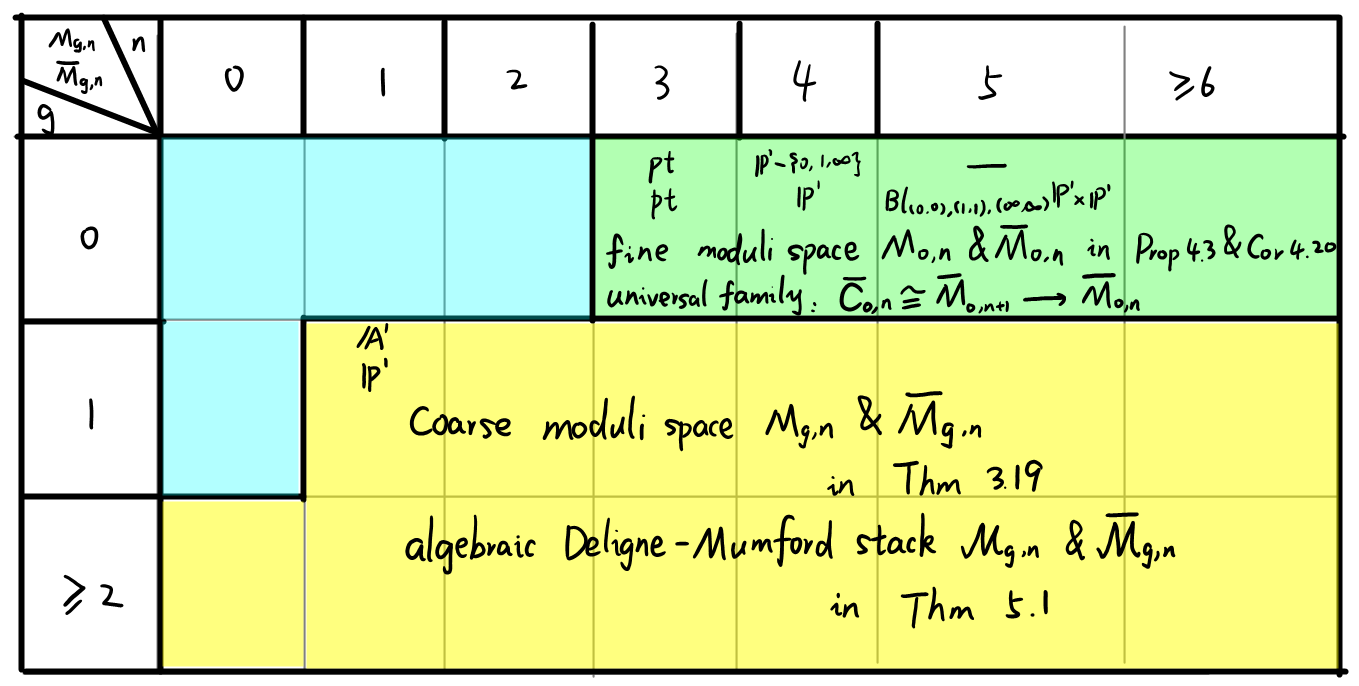
\includegraphics[width=12cm]{figures/moduliofcurve.png}
    \label{fig:moduliofcurve}
    \caption{The moduli of curves}
        
\end{figure} 
%%%%%%%%%%%%%%%%%%%%%%%%%%%%%%%%%%%%%%%%%%%%%%%%%%%%%%%%%%%%%%%%%%%%%%%%%%%%%%%%%%%%%%%%%%%%%
\section{Moduli of elliptic curve}
The elliptic curve theory is especially rich compared to the other curves. That's why we'd like to put it a special section.
\cite[\href{https://stacks.math.columbia.edu/tag/072J}{Tag 072J}]{stacks-project}
\subsection{Differential}
\subsection{Level structure}
\subsection{Complex case}
In this subsection, we will show that how the moduli is connected to the modular curve $\mathcal{H}/\SL_2(\mathbb{Z})$.

%%%%%%%%%%%%%%%%%%%%%%%%%%%%%%%%%%%%%%%%%%%%%%%%%%%%%%%%%%%%%%%%%%%%%%%%%%%%%%%%%%%%%%%%%%%%%
\section{Moduli of vector bundle}
Here we refer to \cite{huybrechts2010geometry}. It's not easy to read, but I don't know the other better reference.
\bibliographystyle{plain}
\bibliography{reference}





\end{document}




